\documentclass[a4paper,12pt, titlepage]{article}
\usepackage[utf8]{inputenc}
\usepackage[english,russian]{babel}
\usepackage{amsmath}
%\usepackage{amsthm}
%\usepackage{cmap}
\usepackage{indentfirst}
\usepackage{a4wide,amssymb}
%\usepackage[pdftex]{graphicx}
%\usepackage[pdftex]{graphics}
%\usepackage{wrapfig}

\usepackage{graphicx}
\renewcommand{\topfraction}{1}
\renewcommand{\textfraction}{0}

%opening
\title{План дипломной работы\\
Коррекция многогранников с помощью локальных деформаций}
\author{Палачев Илья, 510 группа}

\begin{document}

\maketitle
\tableofcontents
%\begin{abstract}
%\end{abstract}


\section{Введение}
\subsection{Происхождение вопроса}
\begin{flushleft}
Данная работа возникла из вопроса автоматизации производственного процесса огранки драгоценных 
камней. 
\end{flushleft}
\begin{flushleft}
Огранка подразумевает создание на поверхности камня ряда геометрически правильных плоскостей, 
граней, от которых будет отражаться попадающий внутрь кристалла свет. После многократного 
внутреннего отражения и преломления лучи света разделяются на спектральные составляющие и, 
покидая камень, создают игру оттенков на его поверхности.
Огранка различается по сложности выполнения. В наиболее сложной и привлекательной бриллиантовой 
огранке может быть до 240 граней. Простая огранка создает на поверхности камня 30 плоскостей.
Качественно выполненная огранка существенно повышает стоимость драгоценного камня, в то же 
время неправильная огранка может «убить» камень, внести в него дефекты. [из Wiki]
\end{flushleft}
\begin{flushleft}
В конечном счете красота бриллианта определяется оптическими свойствами, как присущими 
веществу - алмазу, так и проявляющимися в результате огранки и полировки. Совокупность 
поверхностных и внутренних оптических свойств бриллианта человеческий глаз воспринимает 
как попавшие в глаз разнообразные лучи — белые и цветные, в целом создающие картину 
бриллианта. [из http://3dbook.octonus.com/data/3dbook.html]
\end{flushleft}
\begin{flushleft}
 Форма огранки бриллианта зависит от формы исходного кристалла алмаза. Чтобы получить 
бриллиант максимальной стоимости, огранщики стараются свести к минимуму потери алмаза при обработке. 
В зависимости от формы кристалла алмаза, при его обработке теряется 55—70 \% веса. [из Wiki]
Возможно ли автоматизировать этот процесс? Если да, то насколько? Разница всего в 1/10 карата
может менять стоимость бриллианта в разы.
\end{flushleft}

\subsection{Особенности процесса сканирования алмазов}
\begin{flushleft}
Чтобы автоматизировать процесс огранки, необходимо реализовать построение трехмерных моделей
реальных алмазов. Для их создания используются сканеры, которые фотографируют камень. 
Как это происходит? Камень помещают перед источником света и фотографируют. При этом получается
так называемый \textbf{теневой профиль} камня. Затем камень немного поворачивают и фотографируют 
еще раз. Так делается много раз и в результате на основе фотографий теневого профиля вращающегося
алмаза строится 3D-модель. Опишем этот процесс подробнее.
[http://www.octonus.com/oct/support/doc/scanning.html] 
\end{flushleft}
\begin{flushleft}
 Сначала камень устанавливается на подставке - \textbf{держателе}. Эта подставка вращается и 
периодически производится фотографирование теневого профиля с определенным угловым шагом. Например, в 
сканере алмазов "Helium Polish" фотографирование может производиться в трех режимах 
$[http://www.octonus.com/oct/download/files/Helium\_system\_manual.pdf]$:
\end{flushleft}
\begin{flushleft}
 \begin{tabular}{|p{2.5cm}|p{2.5cm}|p{2.5cm}|p{2.5cm}|p{2.5cm}|}
  \hline
  Метод & Число контуров & Время сканирования, с & Время сборки, с & Полное время, с  \\
  \hline
  Quick & 100 & 12 & 3 & 15 \\
  \hline
  Accuracy & 400 & 47 & 11 & 58 \\
  \hline
  Hi accuracy & 800 & 92 & 30 & 122 \\
  \hline
 \end{tabular}
\end{flushleft}
\begin{flushleft}
 Из этой таблицы видно, что в разных режимах делается от 100 до 800 фотографий одного камня, то есть
модель строится по 100, 400 или 800 теневым контурам. Может ли оказаться так, что два различных камня 
могут быть восприняты системой как одинаковые? Конечно, это возможно, если разница между ними так мала,
что все теневые контуры у них будут идентичны. Всякую модель подобного рода можно понимать как 
пространственное пересечение нескольких бесконечных цилиндров, порожденных теневыми контурами.
\end{flushleft}
\begin{flushleft}
  Может возникнуть коллизия такого рода, когда сам камень имеет какую-то простую структуру, но система
при фотографировании заменяет его на более сложный многогранник. Напимер, модель может иметь такой вид,
как на рис. ~\ref{poly-model}, тогда как в самом деле камень имеет вид, как на рис. ~\ref{poly-real}. Это происходит за счет того, что
угол $\alpha$ между осями проекции очень мал (порядка шага фотографирования).
\end{flushleft}
\begin{flushleft}
  \begin{figure}[h]
    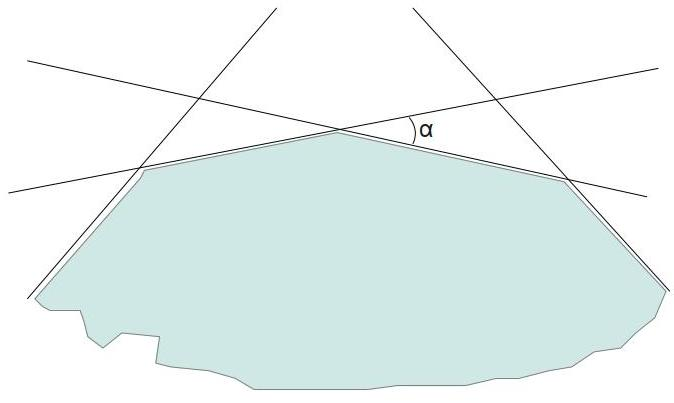
\includegraphics[clip, width=10cm]{img/contour-1.jpg}
    \caption{Смоделированный многогранник}\label{poly-model}
  \end{figure}
  \begin{figure}[h]
    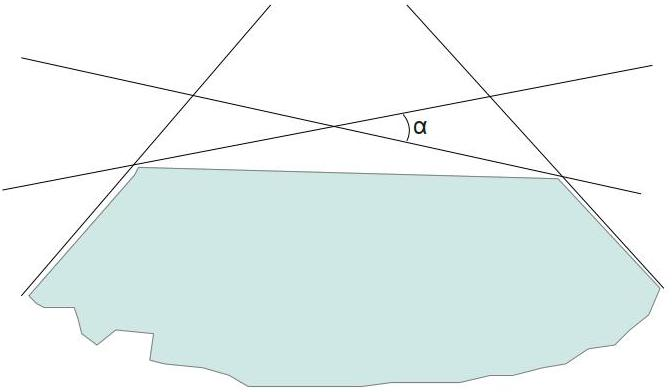
\includegraphics[clip, width=10cm]{img/contour-2.jpg}
    \caption{Реальный камень}\label{poly-real} 
  \end{figure}
\end{flushleft}
\begin{flushleft}
  В таких ситуациях происходит заведомо неоправданное усложнение структуры многогранника. В 3D-моделях
камней происходит разделение крупных граней на 2, 3, 4 более мелких. Это происходит за счет добавления 
в модель несуществующих в камне ребер. Как это может повлиять на дальнейшую работу с моделью? Если идет работа 
с одним камнем, то разница несущественна, но при массовом анализе увеличение числа ребер в 2, 3 раза приводит
к катастрофическому увеличению времени работы алгоритмов. Кроме того, лишние ребра препятствуют анализу характеристик
камня по его модели. Так, если нужно будет найти площадь самой большой грани, то когда в модели эта грань будет 
разделена на 2, то характеристика будет вычислена неверно.
\end{flushleft}
\begin{flushleft}
  Эти соображения и послужили поводом написания данной работы. В ней рассмотрены различные способы коррекции
многогранников при помощи локальных деформаций, без повторного анализа теневых контуров, то есть по уже 
построенной 3D-модели камня.
\end{flushleft}

\subsection{Что понимается под многогранником}
\begin{flushleft}
 Прежде всего следует сказать о том, каким образом задаются многогранники. Во-первых, зададается 
количество вершин и количество граней. Во-вторых, перечисляются координаты всех вершин (это тройки
чисел $x$, $y$, $z$). В-третьих, перечисляются грани. При этом указывается, сколько вершин находится в
грани, в какой плоскости она лежит (четырьмя числами $a$, $b$, $c$, $d$ из уравнения плоскости 
$a x + b y + c z + d = 0$), и список вершин, которые ее составляют.
\end{flushleft}
\begin{flushleft}
  Например, куб с центром в начале координат $(0, 0, 0)$ со сторонами длины 2, параллельными осям
  координат (см. рис. ~\ref{poly-cube}), задается в данной системе следующим образом:
\end{flushleft}
\begin{flushleft}
  \begin{tabular}{|c|c|}
  \hline
    Число вершин & Число граней \\
  \hline
    8 & 6 \\
  \hline 
  \end{tabular}
\end{flushleft}
\begin{flushleft}
  \begin{tabular}{|c|c|c|c|}
    \hline
    Номер вершины & $x$ & $y$ & $z$ \\
    \hline
    0 & -1 & -1 & -1 \\
    1 &  1 & -1 & -1 \\
    2 &  1 &  1 & -1 \\
    3 & -1 &  1 & -1 \\
    4 & -1 & -1 &  1 \\
    5 &  1 & -1 &  1 \\
    6 &  1 &  1 &  1 \\
    7 & -1 &  1 &  1 \\
    \hline
  \end{tabular}
\end{flushleft}
\begin{flushleft}
  \begin{tabular}{|c|c|c|c|c|c|c|}
    \hline
      Номер грани & Число вершин в грани & $a$ & $b$ & $c$ & $d$ & Список вершин \\
    \hline
      0 & 4 &       0 & 0 &-1 &-1&      1, 0, 3, 2 \\
      1 & 4 &       0 &-1 & 0 &-1&      0, 1, 5, 4 \\
      2 & 4 &       1 & 0 & 0 &-1&      1, 2, 6, 5 \\
      3 & 4 &       0 & 1 & 0 &-1&      2, 3, 7, 6 \\
      4 & 4 &      -1 & 0 & 0 &-1&      3, 0, 4, 7 \\
      5 & 4 &       0 & 0 & 1 &-1&      4, 5, 6, 7 \\
    \hline
  \end{tabular}
\end{flushleft}
\begin{flushleft}
  \begin{figure}[h]
    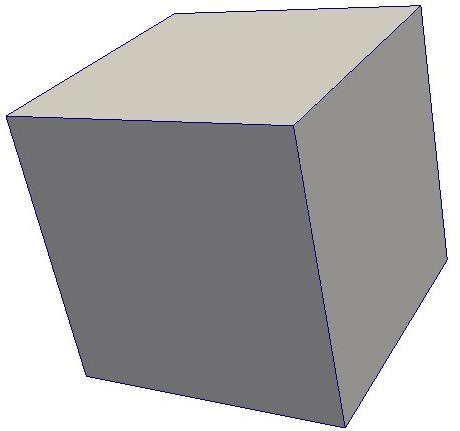
\includegraphics[clip, width=6cm]{img/cube.jpeg}
    \caption{Куб}\label{poly-cube}
  \end{figure}
\end{flushleft}
\begin{flushleft}
 Таким же образом задаются и прочие многогранники
\end{flushleft}




\section{Различные подходы к коррекции многогранников}

\subsection{Подход первый: сечение многогранника плоскостью}
Постановка задачи
\subsubsection{Простейший случай: выпуклый многогранник (сделано - 3 курс)}
Описание алгоритма
\subsubsection{Случай невыпуклого многогранника (сделано - 4 курс)}
Описание алгоритма и демонстрация особых случаев (невуклости, многокомпонентность)

\subsection{Подход второй: сглаживание двух смежных граней}
Постановка задачи
\subsubsection{Построение уравнения новой плоскости методом наименьших квадратов (используется готовый алгоритм)}
Описание алгоритма
\subsubsection{Построение уравнения новой плоскости методом наименьших квадратов с весами}
Имеется в виду, что масса грани должна быть равномерно распределена. В обычном подходе этому
мешают скопления точек, которые вынуждают плоскость пройти близко к ним, увеличивая погрешность
на изолированных точках. Для устранения этого нужно придать изолированным точкам больший вес.
Сделать это можно несколькими способами. \\
	\textbf{1. }Можно считать вес по длинам ребер, исходящих из точки.\\
	\textbf{2. }Можно считать вес по площади (какой?)\\
	\textbf{3. }Может быть, следует обратиться к осям инерции (?).
\subsubsection{Поднятие граней, которые лежат ниже новой плоскости (недоделано - 4 курс)}
При этом возможно два подхода.\\
	\textbf{1. }Строить грани итерационно (обходить контур).\\
	\textbf{2. }Сначала все, что можно поднять - поднимаем, а потом - рассекаем многогранник. Этот подход 
пытался реализовать. Подъем граней должен быть итерационным.

\subsection{Подход второй: подвижка вершины и дальнейшая перестройка многогранника}
\subsubsection{Идея задачи}
\subsubsection{Первый вариант формализации задачи (неудачный)}
Имеется ввиду, что варьируются только координаты вершин. В общем случае система перепределена.
\subsubsection{Второй вариант формализации задачи (неудачный)}
Имеется ввиду, что варьируются и вершины, и грани. Тогда функционал является многочленом четвертой степени 
и его минимизировать проблематично.
\subsubsection{Третий вариант формализации задачи (удачный)}
\begin{flushleft}
Здесь же вариация происходит поочередно:\\
	\textbf{1. }Вычисляем плоскости методом наименьших квадратов\\
	\textbf{2. }Изменяем координаты вершин таким образом, чтобы минимизировать функционал\\
$$	
	\sum\limits_{i = 1}^{N - 1}(|\Delta x_{i}|^{2} + |\Delta y_{i}|^{2} + |\Delta z_{i}|^{2}) + 
	K\sum\limits_{j = 1}^{M}\sum\limits_{i: A_{i} \in \pi_{j}}
	|a_{j}x_{i} + b_{j}y_{i} + c_{j}z_{i} + d_{j}|^{2} \to \min		
$$
При этом нужно помнить, что коэффициенты уравнений плоскостей на этом шаге уже фиксированы, и менять
их не нужно. Переменная $K$ называется штрафом\\
	\textbf{3. }Возвращаемся к пункту 1. и т. д.\\
\end{flushleft}
\begin{flushleft}
Это всего лишь примерный план реализации алгоритма. В действительности есть много его модификаций: от
тех, которые дают довольно адекватный результат, до тех, которые полностью `выворачивают` многогранник 
наизнанку. 
\end{flushleft}
\begin{flushleft}
Множественность возникает из-за того, что задаче есть два изменяемых параметра:\\
	\textbf{1. }Штраф $K$. Каким его сделать? Если слишком большим, то алгоритм перестанет 
'чувствовать' смещения вершин, а если слишком малым, то наооброт - алгоритм будет плохо решать задачу
восстановления плоскостности многогранника.\\
	\textbf{2. }Как чередовать шаги 1 и 2? Менять ли при этом штраф $K$?
\end{flushleft}
\begin{flushleft}
 В результате тестирования наиболее приемлемым оказался следующий подход:\\
	\textbf{1. }$K = 100$\\
	\textbf{2. }$\epsilon = 10^{-7}$\\
	\textbf{3. }Цикл 1. Делать 10 раз:\\
	\textbf{3.1. }Делать цикл 2: \\
	\textbf{3.1.1. }Вычислить новые плоскости методом наименьших квадратов\\
	\textbf{3.1.2. }Вычислить координаты вершин, минимизирующих функционал со штрафом, равным $K$\\
	\textbf{3.2.3. }Вычислить погрешность попадания вершин в плоскости\\
	\textbf{3.2 }...пока эта погрешность больше, чем $\epsilon$\\
	\textbf{3.3 }Конец цикла 2\\
	\textbf{3.4 }Увеличиваем $K$ в два раза\\
	\textbf{3.5 }Уменьшаем $\epsilon$ в два раза\\
	\textbf{4. }Конец цикла 1.\\
\end{flushleft}

\begin{flushleft}
Как этот алгоритм работает? На тестируемых многогранниках он выдал следующее поведение. Программа заходит в цикл 1, затем в нем - 
в цикл 2, делает примерно 30 шагов, выходит из 2 цикла, снова начинает 2 цикл (с увеличенным в 2 раза штрафом и с уменьшенной в 
2 раза погрешностью), но теперь уже делает только 1 шаг, снова выходит из 2 цикла и т. д. - всего примерно 10 раз.
Вот таблица результатов алгоритма ($\Delta$ - сумарный сдвиг вершин, $\epsilon$ - погрешность попадания вершин в плоскости,
$\epsilon_{0}$ - граница погрешности, пересечение которой обеспечивает конец цикла 2, $K$ - штраф):\\
\begin{tabular}{|c|c|c|c|c|c|}
\hline
 цикл 1 & цикл 2 & $\Delta$ & $\epsilon$& $\epsilon_{0}$&  $K$\\
\hline
 0 & 0 & 0.114942 & 4.220043e-02 & 1.000000e-07 & 100.000000\\
\hline
 0 & 1 & 0.048647 & 2.640706e-02 & 1.000000e-07 & 100.000000\\
\hline
 0 & 2 & 0.018739 & 1.637491e-02 & 1.000000e-07 & 100.000000\\
\hline
 0 & 3 & 0.007239 & 1.015491e-02 & 1.000000e-07 & 100.000000\\
\hline
 0 & 4 & 0.002856 & 6.344031e-03 & 1.000000e-07 & 100.000000\\
\hline
 0 & 5 & 0.001151 & 3.991388e-03 & 1.000000e-07 & 100.000000\\
\hline
 0 & 6 & 0.000472 & 2.528785e-03 & 1.000000e-07 & 100.000000\\
\hline
 0 & 7 & 0.000196 & 1.634950e-03 & 1.000000e-07 & 100.000000\\
\hline
 0 & 8 & 0.000082 & 1.064094e-03 & 1.000000e-07 & 100.000000\\
\hline
 0 & 9 & 0.000035 & 6.940496e-04 & 1.000000e-07 & 100.000000\\
\hline
 0 & 10 & 0.000015 & 4.535194e-04 & 1.000000e-07 & 100.000000\\
\hline
 0 & 11 & 0.000006 & 2.967911e-04 & 1.000000e-07 & 100.000000\\
\hline
 0 & 12 & 0.000003 & 1.944614e-04 & 1.000000e-07 & 100.000000\\
\hline
 0 & 13 & 0.000001 & 1.275375e-04 & 1.000000e-07 & 100.000000\\
\hline
 0 & 14 & 0.000001 & 8.370982e-05 & 1.000000e-07 & 100.000000\\
\hline
 0 & 15 & 0.000000 & 5.497753e-05 & 1.000000e-07 & 100.000000\\
\hline
 0 & 16 & 0.000000 & 3.612497e-05 & 1.000000e-07 & 100.000000\\
\hline
 0 & 17 & 0.000000 & 2.374594e-05 & 1.000000e-07 & 100.000000\\
\hline
 0 & 18 & 0.000000 & 1.561315e-05 & 1.000000e-07 & 100.000000\\
\hline
 0 & 19 & 0.000000 & 1.026795e-05 & 1.000000e-07 & 100.000000\\
\hline
 0 & 20 & 0.000000 & 6.753804e-06 & 1.000000e-07 & 100.000000\\
\hline
 0 & 21 & 0.000000 & 4.442928e-06 & 1.000000e-07 & 100.000000\\
\hline
 0 & 22 & 0.000000 & 2.923018e-06 & 1.000000e-07 & 100.000000\\
\hline
 0 & 23 & 0.000000 & 1.923204e-06 & 1.000000e-07 & 100.000000\\
\hline
 0 & 24 & 0.000000 & 1.265446e-06 & 1.000000e-07 & 100.000000\\
\hline
 0 & 25 & 0.000000 & 8.326840e-07 & 1.000000e-07 & 100.000000\\
\hline
 0 & 26 & 0.000000 & 5.479375e-07 & 1.000000e-07 & 100.000000\\
\hline
 0 & 27 & 0.000000 & 3.605724e-07 & 1.000000e-07 & 100.000000\\
\hline
 0 & 28 & 0.000000 & 2.372805e-07 & 1.000000e-07 & 100.000000\\
\hline
 0 & 29 & 0.000000 & 1.561485e-07 & 1.000000e-07 & 100.000000\\
\hline
 0 & 30 & 0.000000 & 1.027587e-07 & 1.000000e-07 & 100.000000\\
\hline
 0 & 31 & 0.000000 & 6.762423e-08 & 1.000000e-07 & 100.000000\\
\hline
 1 & 32 & 0.000000 & 2.585086e-08 & 5.000000e-08 & 200.000000\\
\hline
 2 & 33 & 0.000000 & 9.229164e-09 & 2.500000e-08 & 400.000000\\
\hline
 3 & 34 & 0.000000 & 3.159339e-09 & 1.250000e-08 & 800.000000\\
\hline
 4 & 35 & 0.000000 & 1.053913e-09 & 6.250000e-09 & 1600.000000\\
\hline
 5 & 36 & 0.000000 & 3.462331e-10 & 3.125000e-09 & 3200.000000\\
\hline
 6 & 37 & 0.000000 & 1.131674e-10 & 1.562500e-09 & 6400.000000\\
\hline
 7 & 38 & 0.000000 & 3.720410e-11 & 7.812500e-10 & 12800.000000\\
\hline
 8 & 39 & 0.000000 & 1.253741e-11 & 3.906250e-10 & 25600.000000\\
\hline
 9 & 40 & 0.000000 & 4.448228e-12 & 1.953125e-10 & 51200.000000\\
\hline
\end{tabular}
\end{flushleft}
Нужно реализовать следующие идеи:\\
	\textbf{1. }Попробовать разную динамику изменения штрафа. Не только 
экспоненциальный рост, но и линейный, логарифмический...\\
	\textbf{2. }Решить проблему ``выворачивания'' многогранника. Дело в том, что если 
начальная деформация точки слишком велика, то нарушается корректность многогранника 
(грани выворачиваются или наезжают друг на друга). В продемонстрированном выше примере точка двигалась
на расстояние порядка 0.1, тогда как одно из ребер, из нее исходящих, имеет длину порядка 0.03. 
Вот что при этом наблюдается:\\
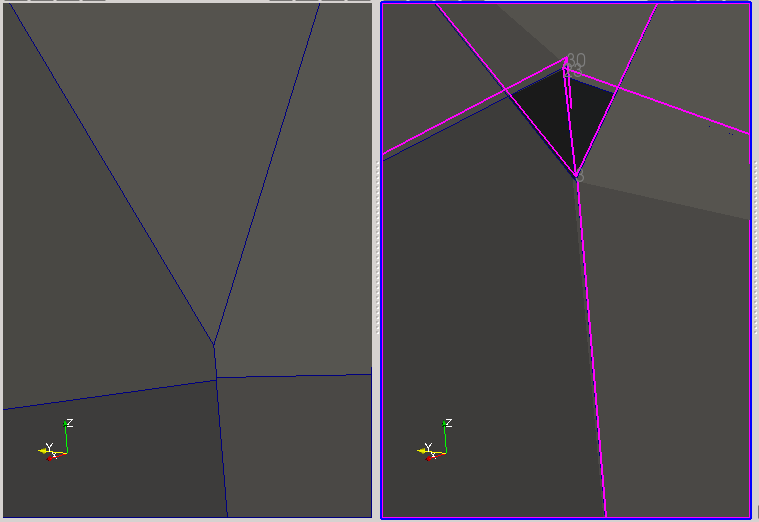
\includegraphics[clip, width=15cm]{img/2-1.png}
При решении проблемы выворачнивания нужно решить, вообще говоря, три задачи:\\
	\textbf{2.1. }На какое максимальное расстояние расстояние можно двигать точку, не изменяя при этом топологической структуры 
многогранника?\\
	\textbf{2.2. }Попытаться делать деформацию не разом за одно применение программы, а, скажем, делить вектор сдвига на 10 частей
и за 10 применений программы реализовать сдвиг.\\
	\textbf{2.3. }Если эти две задачи решены, то может быть попытаться решить задачу, когда сдвиг больше допустимого, то есть когда
мы сначала сдвигаем точку на максимально допустимое расстояние, затем меняем немного структуру многогранника, а затем сдвигаем еще раз.
(???)

\subsubsection{Анализ сходимости и трудоемкости алгоритма}
Про сходимость алгоритма до сих пор ничего не известно, доказать не удалось.
(TODO)
\end{document}
